\section*{Приложение А}
\addcontentsline{toc}{section}{Приложение А}

\begin{sidewaysfigure}[h]
	\centering
	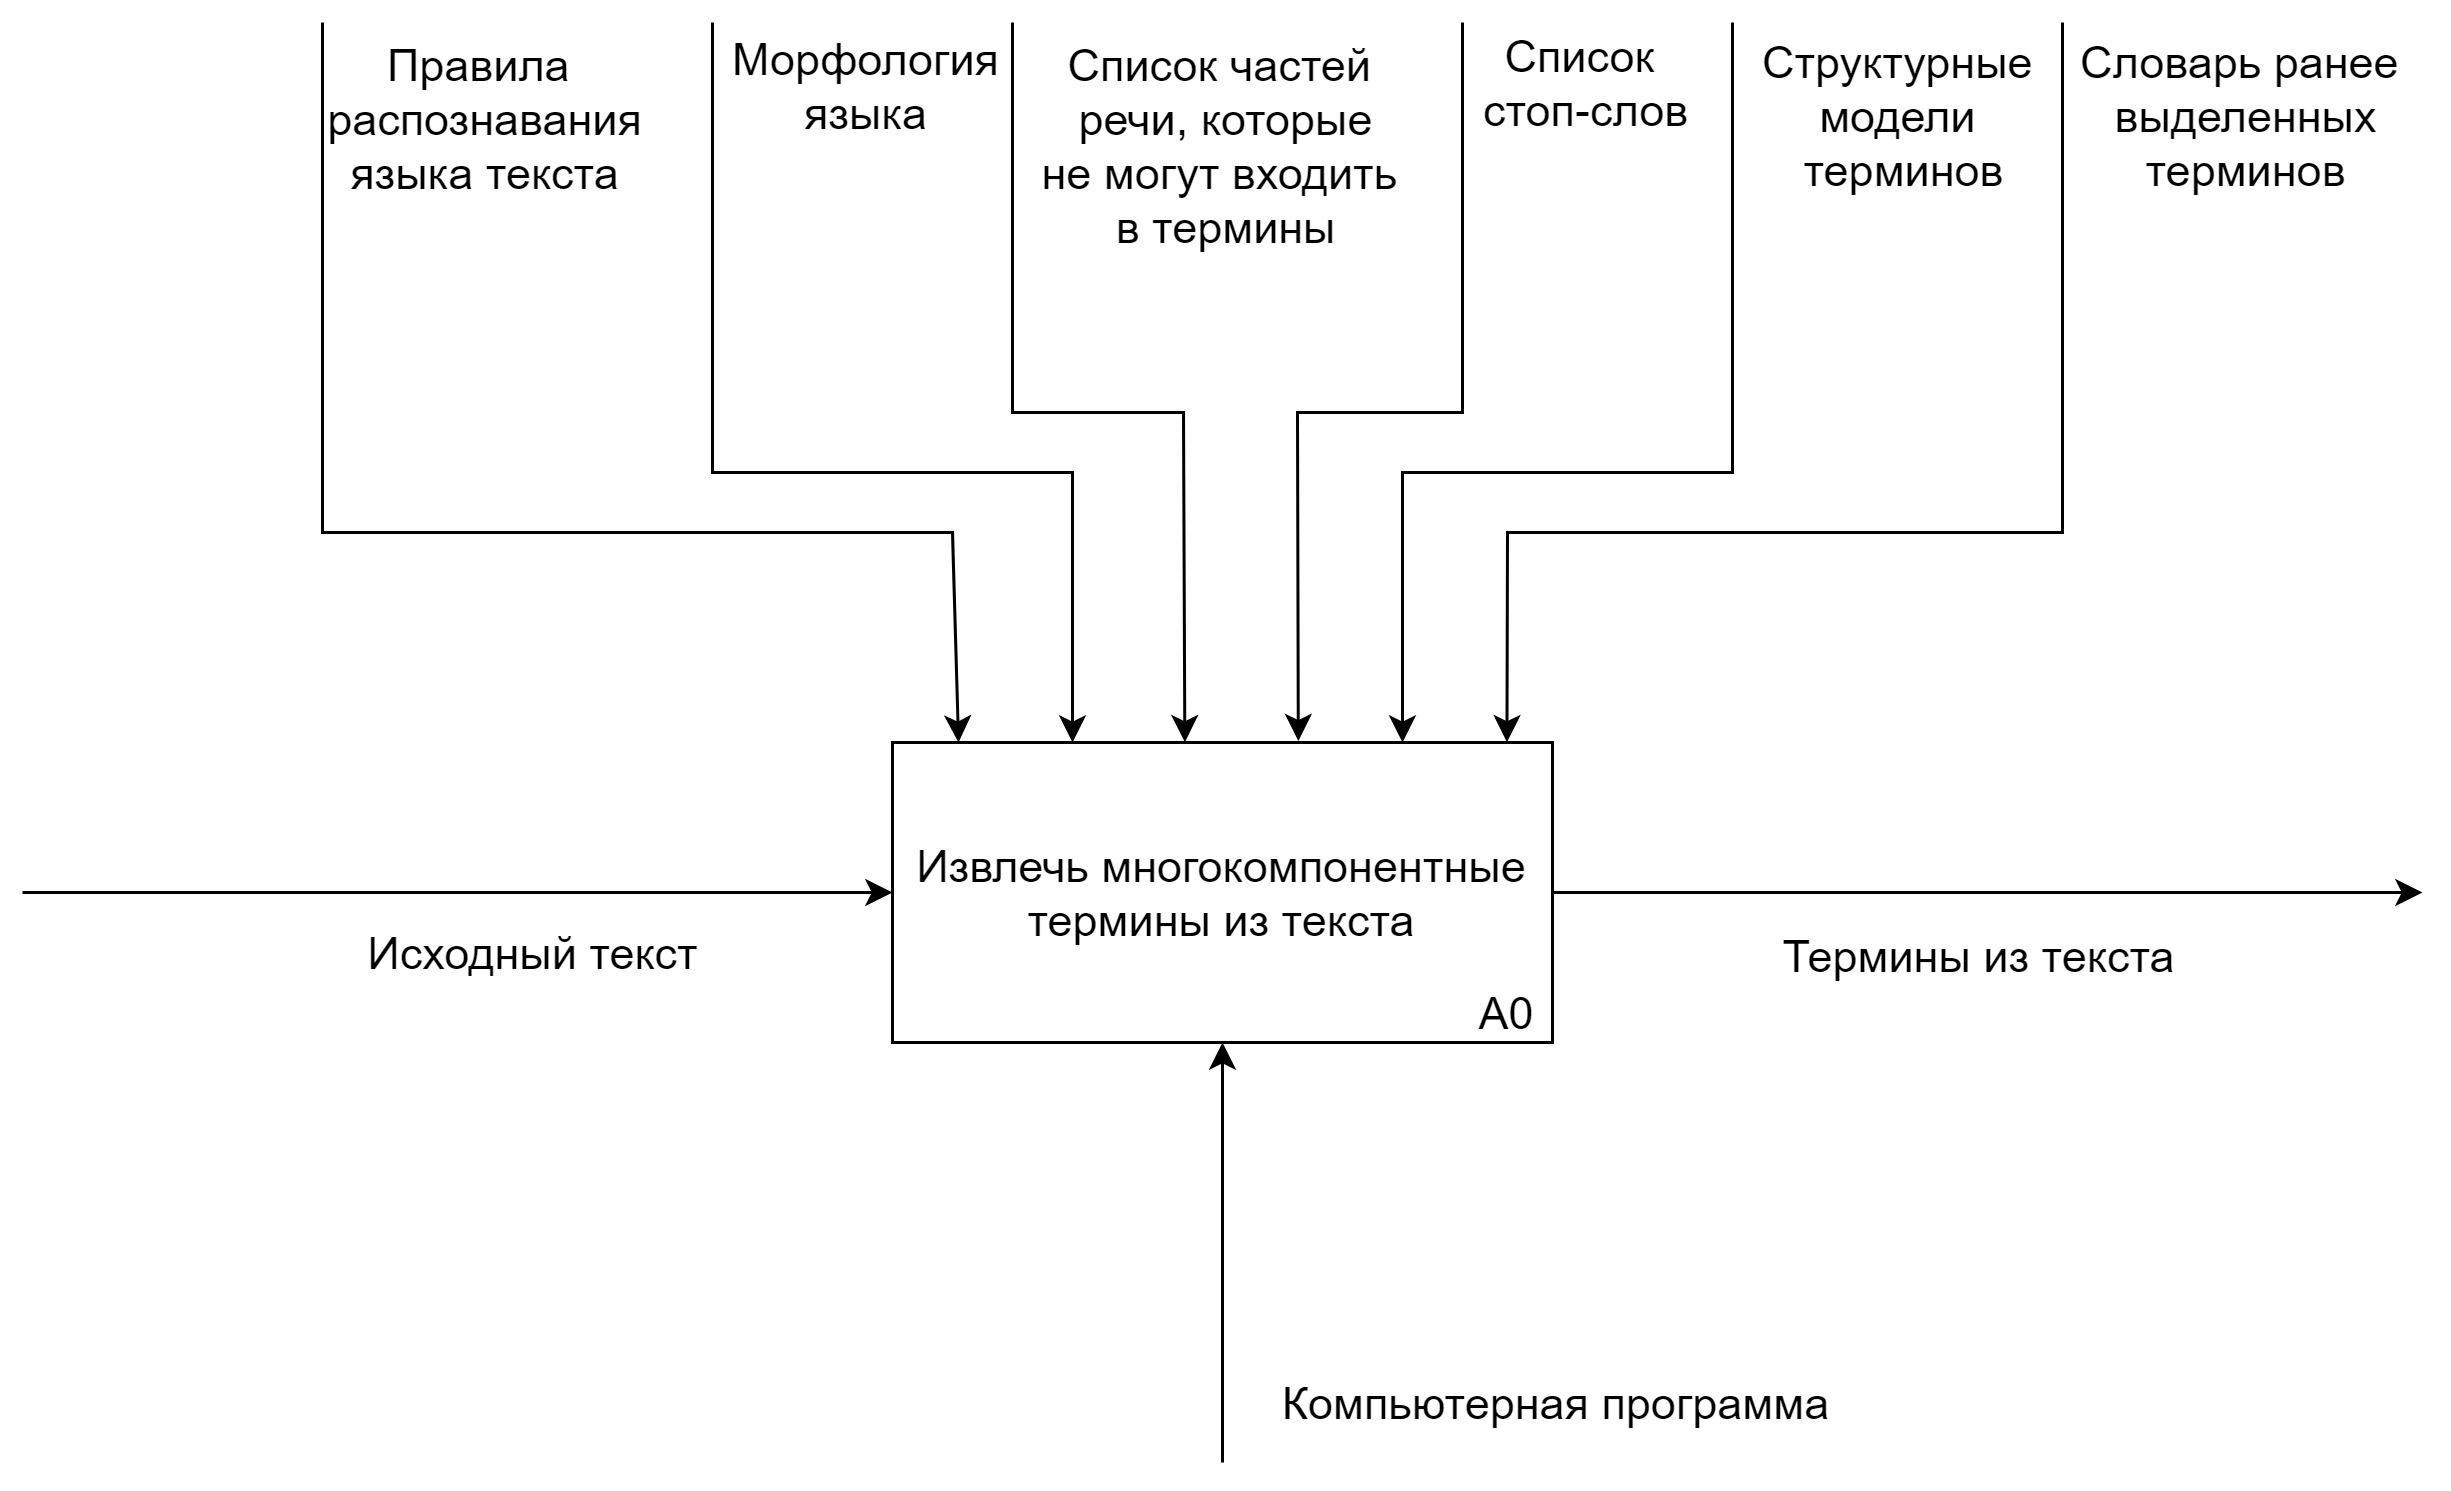
\includegraphics[width=0.83\textwidth ]{img/IDEF0/A0.png}
	\caption{Функциональная схема работы системы извлечения многокомпонентных терминов, верхний уровень}
\end{sidewaysfigure} 

\begin{sidewaysfigure}[h]
	\centering
	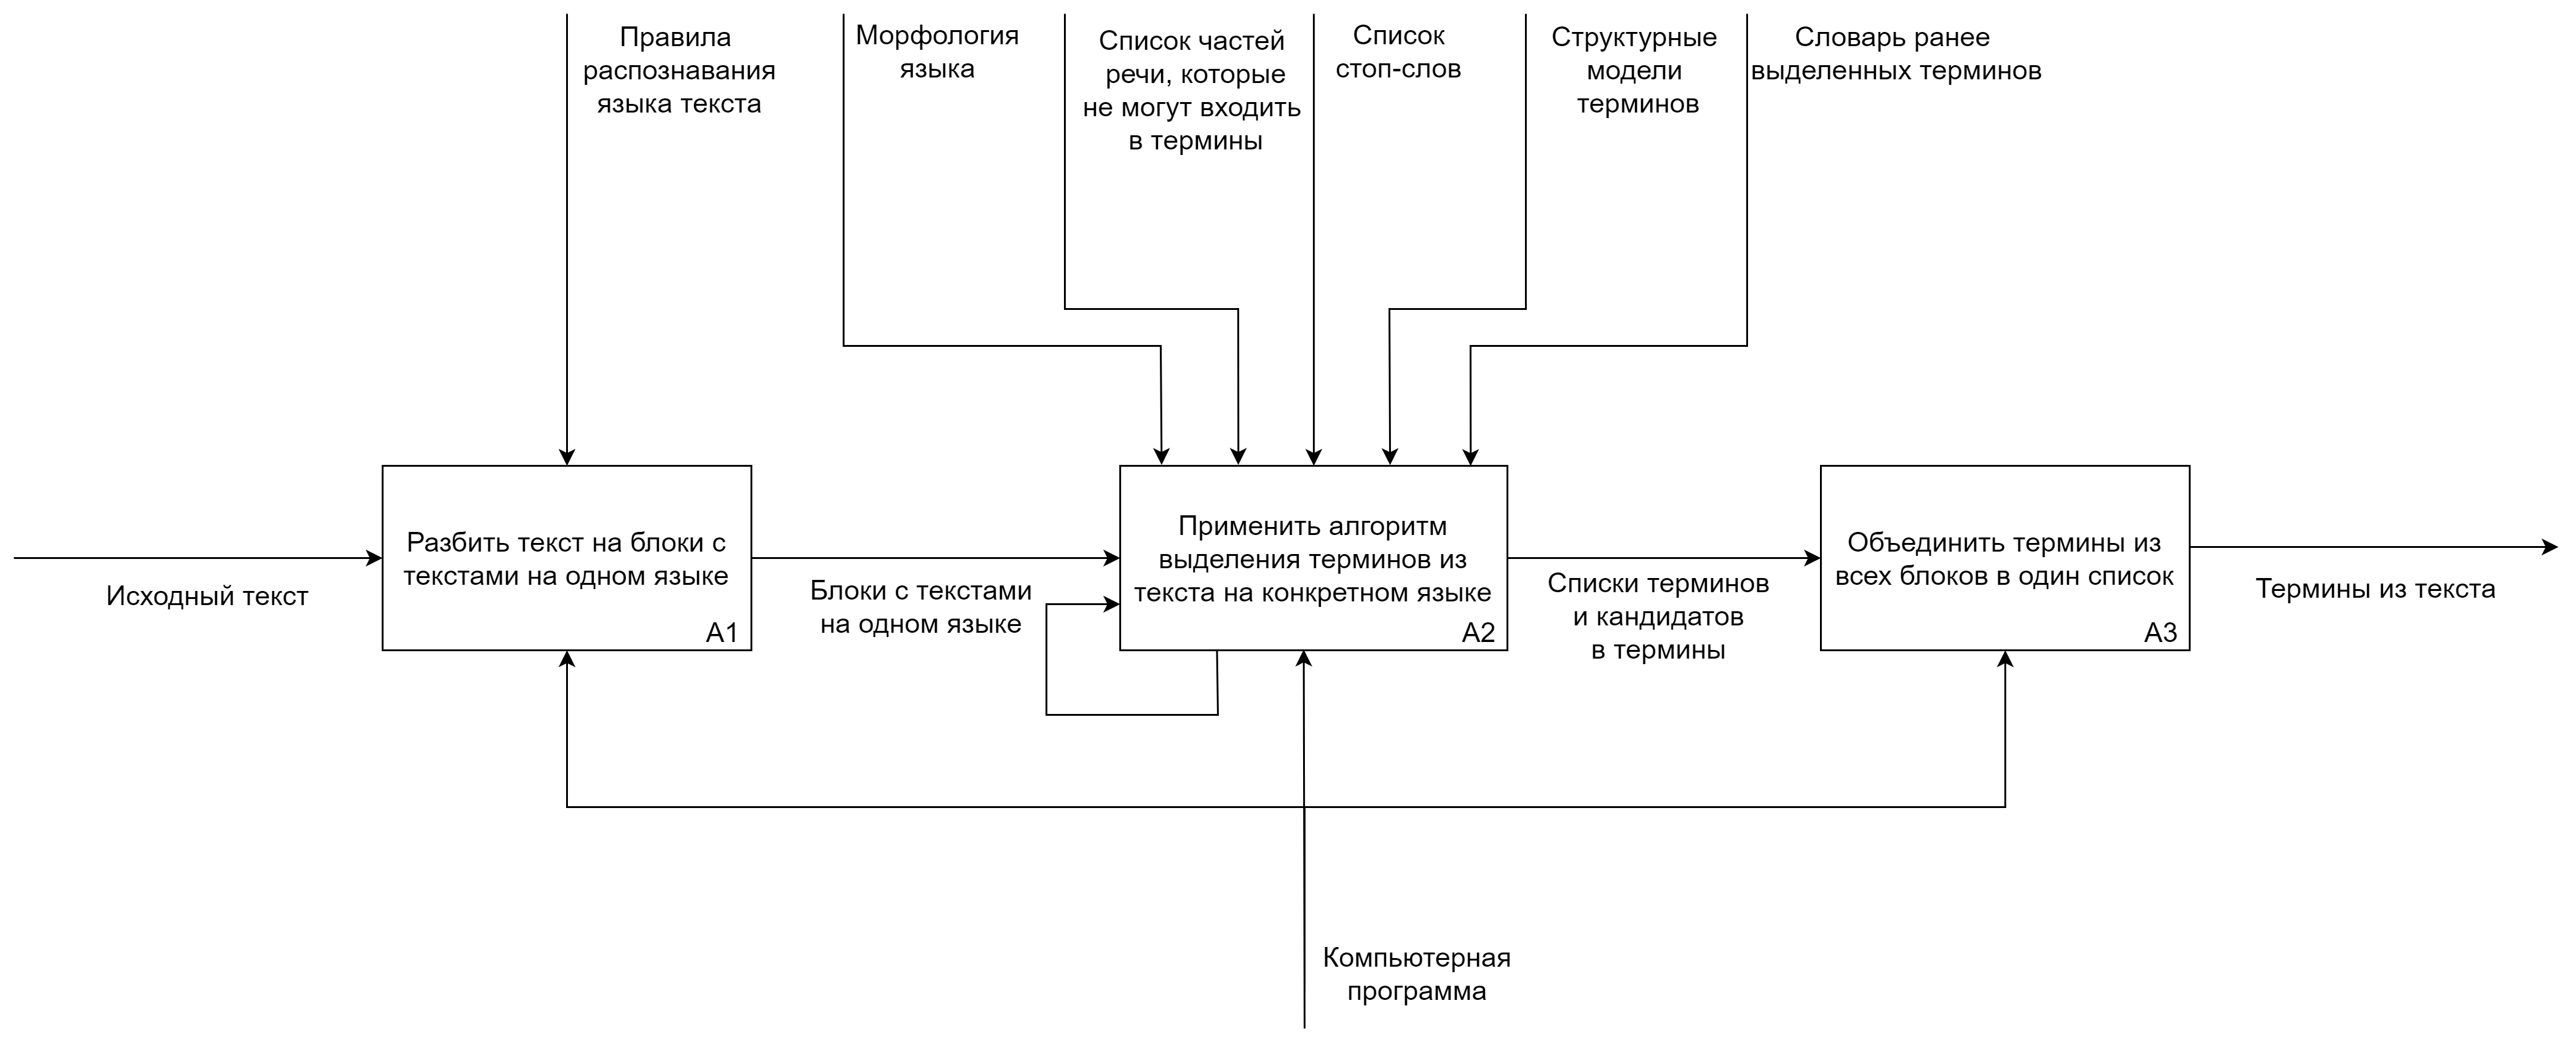
\includegraphics[width=\textwidth ]{img/IDEF0/A0_decomposition.png}
	\caption{Функциональная схема работы системы извлечения многокомпонентных терминов, декомпозиция уровня A0}
\end{sidewaysfigure} 

\begin{sidewaysfigure}[h]
	\centering
	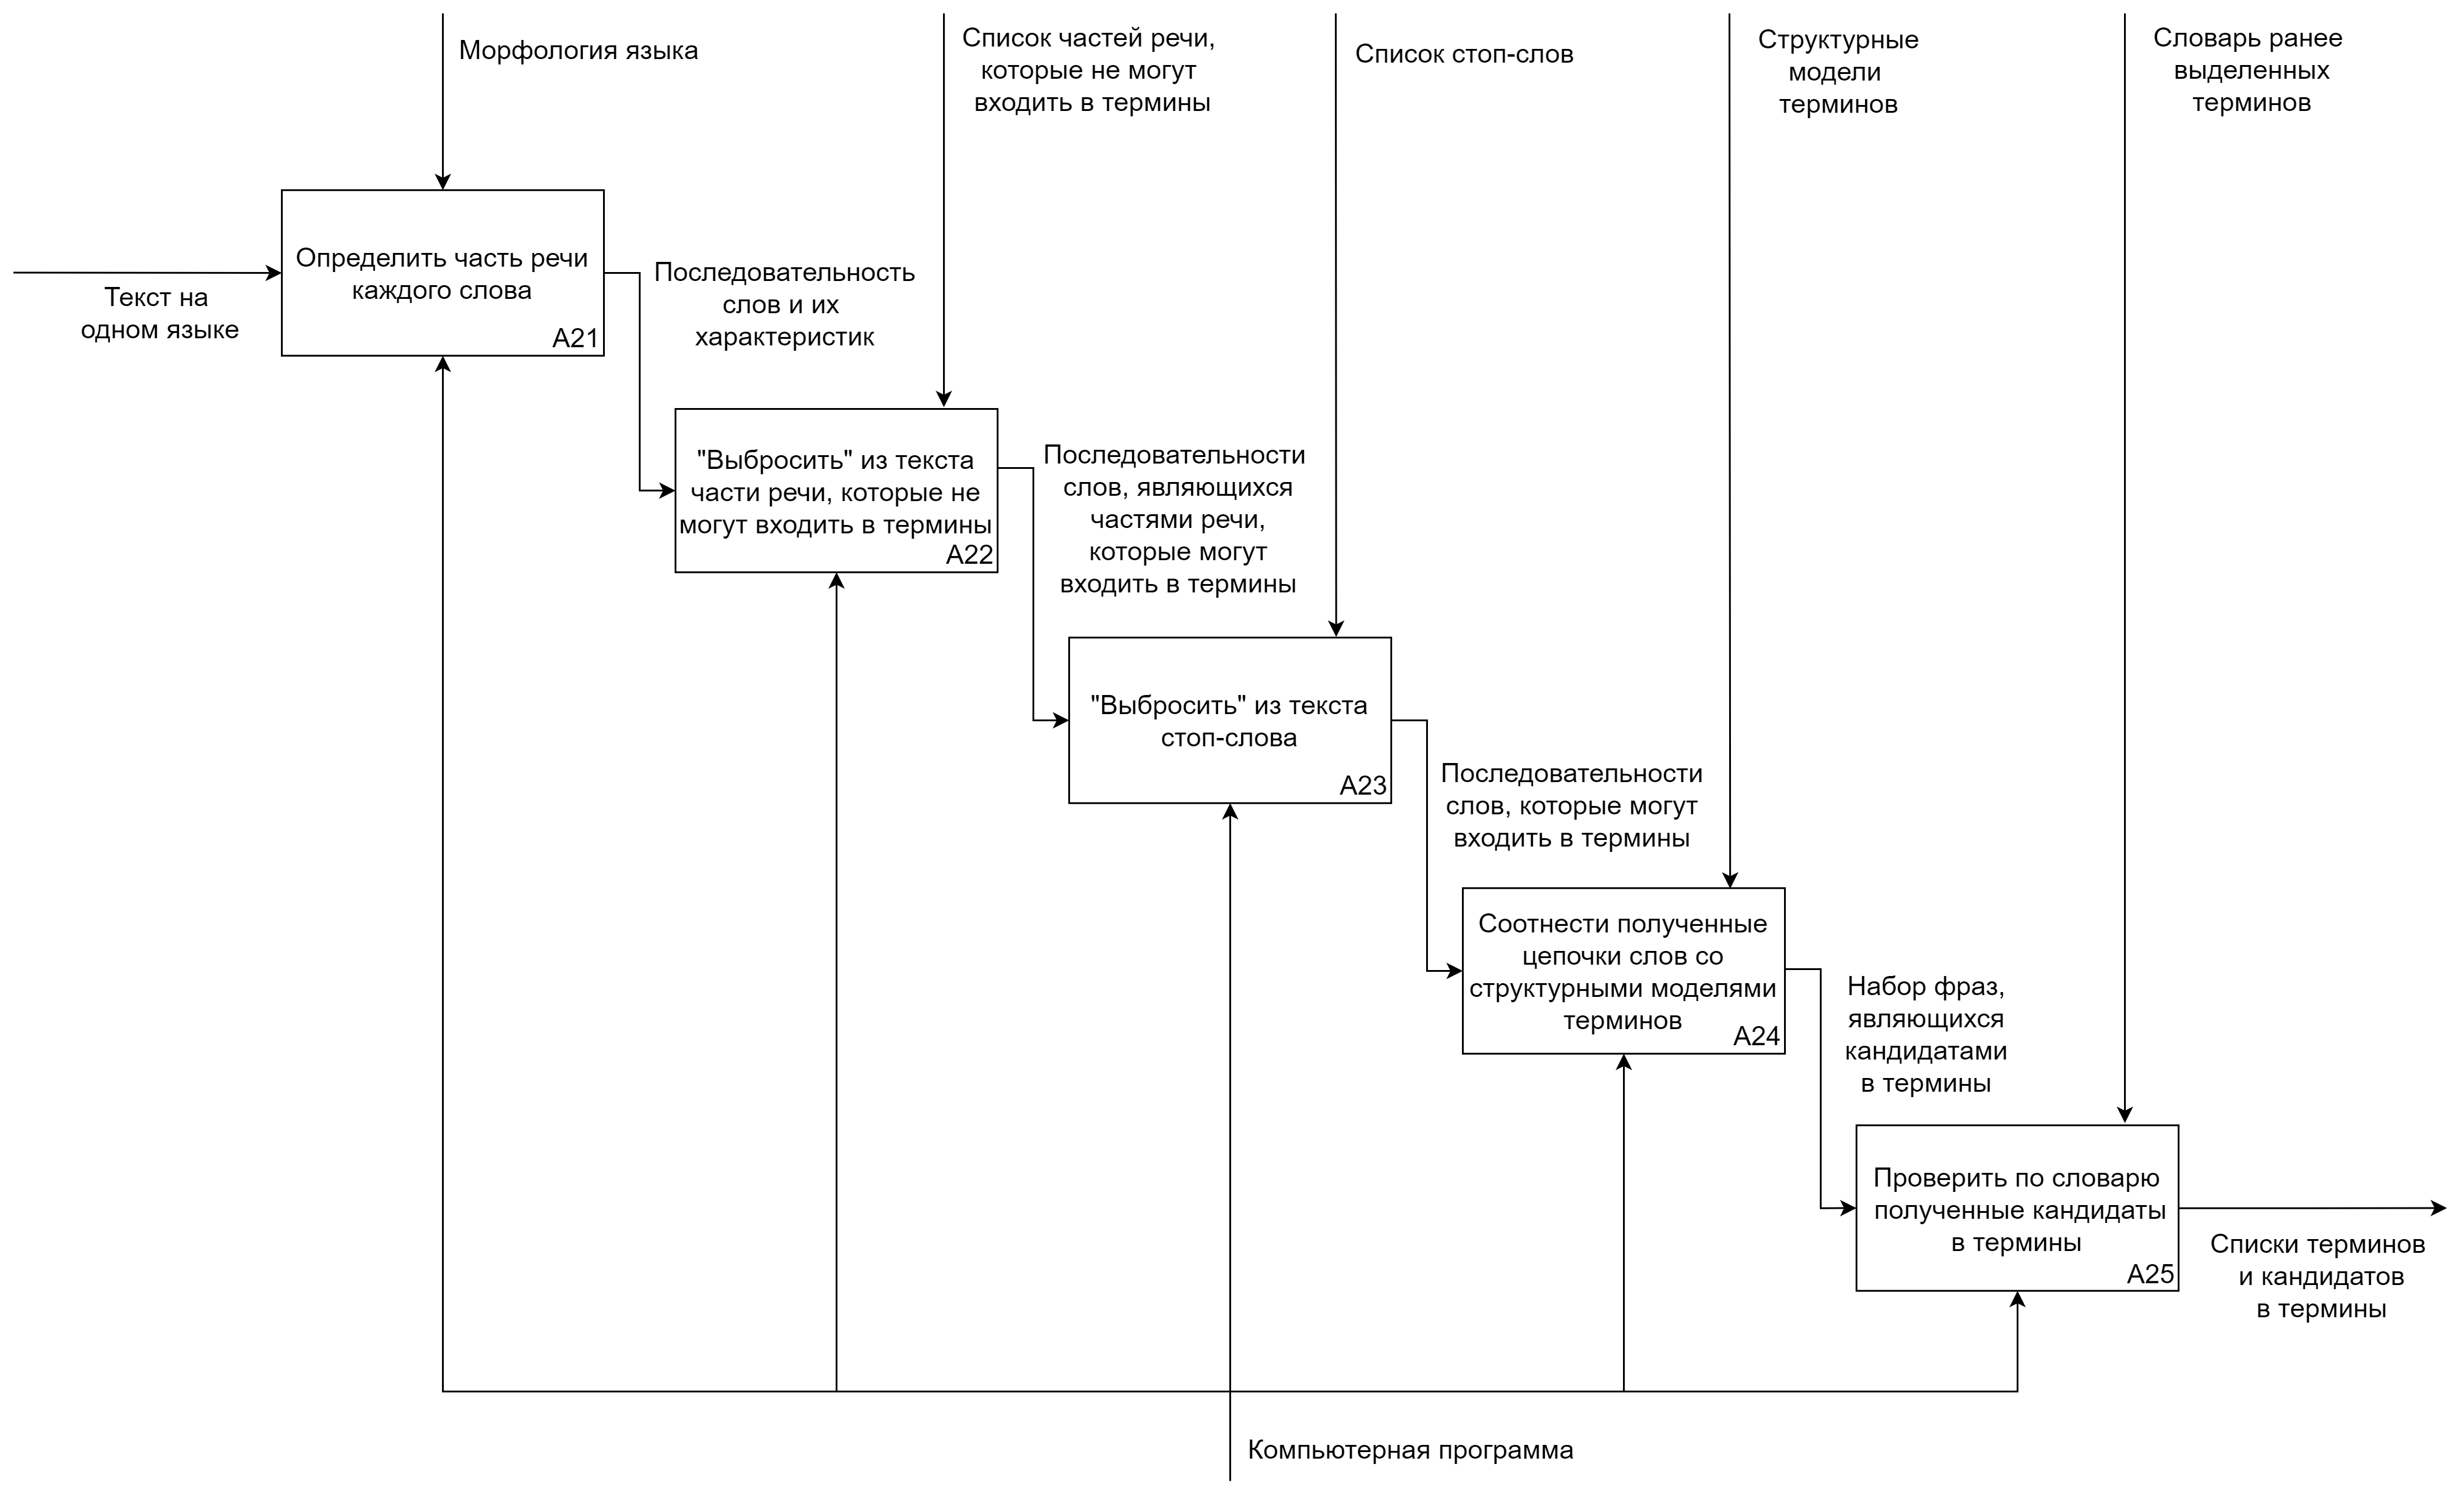
\includegraphics[width=\textwidth ]{img/IDEF0/A2_decomposition.png}
	\caption{Функциональная схема работы системы извлечения многокомпонентных терминов, декомпозиция уровня A2}
\end{sidewaysfigure} 

\pagebreak